\documentclass[12pt, a4paper]{book}

\usepackage[T1]{fontenc}
\usepackage[utf8]{inputenc}
\usepackage[charter, cal=cmcal]{mathdesign}
\usepackage[scaled=0.92]{helvet}
\usepackage{geometry}
\geometry{a4paper, top=30mm, bottom=30mm, inner=32mm, outer=25mm, marginparwidth=18mm}

\usepackage{amsmath, amsthm}
\usepackage[version=4]{mhchem}
\usepackage{graphicx}
\usepackage[dvipsnames,svgnames,table]{xcolor}
\usepackage{tikz}
\usetikzlibrary{arrows.meta, shapes.geometric, positioning,
                calc, backgrounds, decorations.pathmorphing, patterns}
\usepackage{pgfplots}
\pgfplotsset{compat=1.18}
\usepackage{tcolorbox}
\tcbuselibrary{skins, breakable, theorems}
\usepackage{titlesec}
\usepackage{fancyhdr}
\usepackage{enumitem}
\usepackage{booktabs}
\usepackage{array}
\usepackage{multicol}
\usepackage{caption}
\usepackage{parskip}
\usepackage{siunitx}
\usepackage{pifont}
\usepackage[colorlinks=true, linkcolor=BrickRed,
            urlcolor=NavyBlue, citecolor=ForestGreen]{hyperref}

% ── Colours ───────────────────────────────────────────────────────────────────
\definecolor{JourneyColor}{HTML}{4A235A}
\definecolor{ModuleColor}{HTML}{6C3483}
\definecolor{PuzzleColor}{HTML}{1A5276}
\definecolor{DiscoveryColor}{HTML}{B7950B}
\definecolor{WarningColor}{HTML}{C0392B}
\definecolor{ProblemColor}{HTML}{117A65}
\definecolor{ReflectColor}{HTML}{1D6A39}
\definecolor{HistoryColor}{HTML}{6E2F1A}
\definecolor{LightBg}{HTML}{F8F9FA}
\definecolor{ElectronBlue}{HTML}{1565C0}
\definecolor{NucleusRed}{HTML}{B71C1C}
\definecolor{blue!50!red}{HTML}{5E35B1}
\definecolor{red}{HTML}{D32F2F}
\definecolor{cyan!80!black}{HTML}{00838F}
\definecolor{blue}{HTML}{1565C0}

% ── Boxes ─────────────────────────────────────────────────────────────────────
\newtcolorbox{puzzlebox}[1][]{enhanced,breakable,
  colback=PuzzleColor!6,colframe=PuzzleColor,fonttitle=\bfseries\sffamily,
  title={The Puzzle},attach boxed title to top left={yshift=-2mm,xshift=6mm},
  boxed title style={colback=PuzzleColor},borderline west={3pt}{0pt}{PuzzleColor},#1}

\newtcolorbox{discoverybox}[1][]{enhanced,breakable,
  colback=DiscoveryColor!8,colframe=DiscoveryColor,fonttitle=\bfseries\sffamily,
  title={Discovery},attach boxed title to top left={yshift=-2mm,xshift=6mm},
  boxed title style={colback=DiscoveryColor},borderline west={3pt}{0pt}{DiscoveryColor},#1}

\newtcolorbox{problembox}[1][]{enhanced,breakable,
  colback=ProblemColor!5,colframe=ProblemColor,fonttitle=\bfseries\sffamily,
  title={Problems},attach boxed title to top left={yshift=-2mm,xshift=6mm},
  boxed title style={colback=ProblemColor},borderline west={3pt}{0pt}{ProblemColor},#1}

\newtcolorbox{deepbox}[1][]{enhanced,breakable,
  colback=JourneyColor!5,colframe=JourneyColor,fonttitle=\bfseries\sffamily,
  title={Deep Problems},attach boxed title to top left={yshift=-2mm,xshift=6mm},
  boxed title style={colback=JourneyColor},borderline west={4pt}{0pt}{JourneyColor},#1}

\newtcolorbox{historybox}[1][]{enhanced,breakable,
  colback=HistoryColor!7,colframe=HistoryColor!60,fonttitle=\bfseries\sffamily\small,
  title={Historical Note},attach boxed title to top left={yshift=-2mm,xshift=6mm},
  boxed title style={colback=HistoryColor!80},#1}

\newtcolorbox{reflectionbox}[1][]{enhanced,breakable,
  colback=ReflectColor!6,colframe=ReflectColor,fonttitle=\bfseries\sffamily,
  title={Reflection},attach boxed title to top left={yshift=-2mm,xshift=6mm},
  boxed title style={colback=ReflectColor},borderline west={3pt}{0pt}{ReflectColor},#1}

\newtcolorbox{modelbreaks}[1][]{enhanced,breakable,
  colback=WarningColor!6,colframe=WarningColor,fonttitle=\bfseries\sffamily,
  title={Where This Model Breaks},attach boxed title to top left={yshift=-2mm,xshift=6mm},
  boxed title style={colback=WarningColor},borderline west={4pt}{0pt}{WarningColor},#1}

\newtcolorbox{namedconcept}[2][]{enhanced,
  colback=ModuleColor!6,colframe=ModuleColor,fonttitle=\bfseries\sffamily\large,
  title={#2},attach boxed title to top left={yshift=-2mm,xshift=6mm},
  boxed title style={colback=ModuleColor},#1}

% ── Section formatting ────────────────────────────────────────────────────────
\titleformat{\chapter}[display]
  {\normalfont\sffamily\huge\bfseries\color{JourneyColor}}
  {\textcolor{JourneyColor!60}{\chaptertitlename\ \thechapter}}{10pt}{\Huge}
  [\vspace{2pt}\textcolor{JourneyColor}{\titlerule[1.5pt]}]
\titleformat{\section}
  {\normalfont\sffamily\Large\bfseries\color{ModuleColor}}
  {\thesection}{1em}{}[\textcolor{ModuleColor!40}{\titlerule[0.6pt]}]
\titleformat{\subsection}
  {\normalfont\sffamily\large\bfseries\color{JourneyColor!80}}{\thesubsection}{1em}{}
\titleformat{\subsubsection}
  {\normalfont\sffamily\normalsize\bfseries}{\thesubsubsection}{1em}{}

\pagestyle{fancy}
\fancyhf{}
\fancyhead[LE]{\small\sffamily\textcolor{JourneyColor}{\leftmark}}
\fancyhead[RO]{\small\sffamily\textcolor{ModuleColor}{\rightmark}}
\fancyfoot[C]{\small\thepage}
\renewcommand{\headrulewidth}{0.4pt}

\newcommand{\newterm}[1]{\textit{\textcolor{DiscoveryColor}{#1}}}
\newcommand{\important}[1]{\textcolor{ModuleColor}{\textbf{#1}}}

% ══════════════════════════════════════════════════════════════════════════════
\begin{document}
\setcounter{chapter}{1}
\chapter[Journey 2 --- Architecture of the Atom]
        {Journey Two\\[8pt]
         \textcolor{ModuleColor}{\large Architecture of the Atom}}
\setcounter{section}{3}

% ══════════════════════════════════════════════════════════════════════════════
\section{Module 2.4 --- The Hydrogen Spectrum and the Birth of Quantisation}
\label{sec:mod2.4}

\subsection*{Motivation}

Classical physics predicts that an atom spiralling to collapse
would emit a continuous spectrum --- a smooth sweep of all colours,
getting brighter at higher frequencies as the electron
speeds up on its way in.

What experimenters actually saw was the opposite of this.

When hydrogen gas is excited by an electrical discharge,
it emits light at a small number of very specific,
very sharp wavelengths.
Nothing else.
No continuum.
No smooth variation.
Just a discrete set of coloured lines.

These lines had been measured with extraordinary precision
since the 1860s.
Their wavelengths were known to six significant figures.
Yet nobody could explain why hydrogen should emit light
at \emph{those particular} wavelengths and no others.

The explanation would require the quantum.

% ─── Section: The Spectrum ───────────────────────────────────────────────────
\subsection{What a Spectrum Is}

When white light passes through a prism, it separates into
a rainbow --- a \newterm{continuous spectrum} containing
all visible wavelengths.

When light from a hot gas passes through a prism,
something completely different appears:
a \newterm{line spectrum} --- a series of bright coloured lines
on a dark background, each at a specific wavelength.

Every element has its own unique line spectrum,
as distinctive as a fingerprint.

\begin{center}
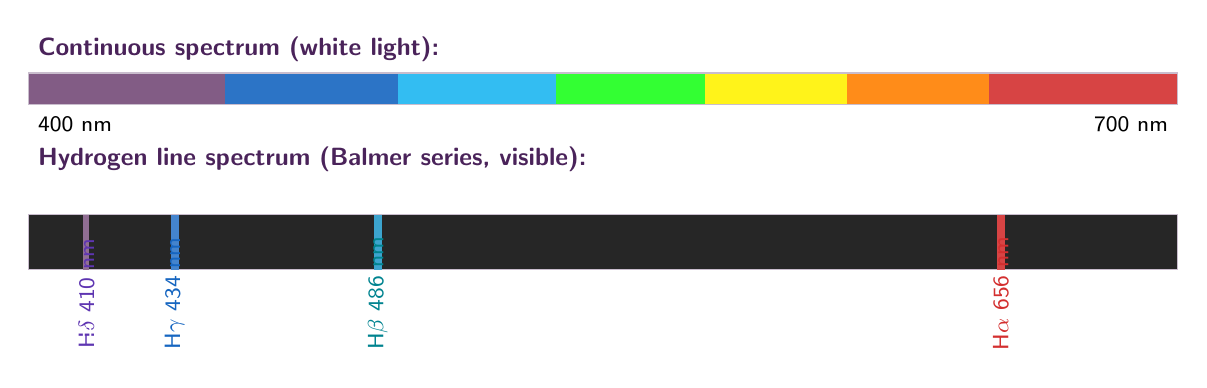
\begin{tikzpicture}[every node/.style={font=\sffamily\footnotesize},
                    scale=1.0]

  % ── Continuous spectrum bar ──────────────────────────────────────────────
  \node[font=\sffamily\small\bfseries, color=JourneyColor, anchor=west]
    at (-0.2, 3.4) {Continuous spectrum (white light):};

  % Approximate rainbow using fixed colour bands
  \fill[blue!50!red!90]   (-0.2,2.7)  rectangle (2.3, 3.1);
  \fill[blue!90]     (2.3, 2.7)  rectangle (4.5, 3.1);
  \fill[cyan!80]     (4.5, 2.7)  rectangle (6.5, 3.1);
  \fill[green!80]    (6.5, 2.7)  rectangle (8.4, 3.1);
  \fill[yellow!90]   (8.4, 2.7)  rectangle (10.2,3.1);
  \fill[orange!90]   (10.2,2.7)  rectangle (12.0,3.1);
  \fill[red!90]      (12.0,2.7)  rectangle (14.4,3.1);
  \draw[JourneyColor!30] (-0.2,2.7) rectangle (14.4,3.1);
  \node[anchor=west] at (-0.2, 2.45) {400 nm};
  \node[anchor=east] at (14.4,  2.45) {700 nm};

  % ── Hydrogen line spectrum ───────────────────────────────────────────────
  \node[font=\sffamily\small\bfseries, color=JourneyColor, anchor=west]
    at (-0.2, 2.0) {Hydrogen line spectrum (Balmer series, visible):};

  % Dark background
  \fill[black!85] (-0.2, 0.6) rectangle (14.4, 1.3);
  \draw[JourneyColor!30] (-0.2,0.6) rectangle (14.4,1.3);

  % Helper: map wavelength (nm) to x position across 400..700 nm range
  % x = (lambda - 400) / 300 * 14.6 - 0.2
  % H-alpha 656.3 nm -> red
  \pgfmathsetmacro{\xHa}{(\the\numexpr656\relax - 400)/300*14.6-0.2}
  \fill[red!90] (12.10, 0.6) rectangle (12.20, 1.3);
  \node[red, rotate=90] at (12.15, 0.3) {H$\alpha$ 656 nm};

  % H-beta 486.1 nm -> cyan-green
  \fill[cyan!80!black!90] (4.19, 0.6) rectangle (4.29, 1.3);
  \node[cyan!80!black, rotate=90] at (4.24, 0.3) {H$\beta$ 486 nm};

  % H-gamma 434.0 nm -> blue!50!red-blue
  \fill[blue!80] (1.61, 0.6) rectangle (1.71, 1.3);
  \node[blue, rotate=90] at (1.66, 0.3) {H$\gamma$ 434 nm};

  % H-delta 410.2 nm -> deep blue!50!red
  \fill[blue!50!red!80] (0.50, 0.6) rectangle (0.57, 1.3);
  \node[blue!50!red, rotate=90] at (0.54, 0.3) {H$\delta$ 410 nm};

  \node[anchor=west, text=white!70] at (-0.2, -0.15) {400 nm};
  \node[anchor=east, text=white!70] at (14.4, -0.15) {700 nm};

\end{tikzpicture}
\end{center}

\vspace{0.8em}

The four visible lines of hydrogen are:
\begin{center}
\begin{tabular}{llll}
\toprule
Line & Wavelength & Colour & Name \\
\midrule
H$\alpha$ & 656.3 nm & Red       & Balmer alpha \\
H$\beta$  & 486.1 nm & Blue-green & Balmer beta \\
H$\gamma$ & 434.0 nm & Violet    & Balmer gamma \\
H$\delta$ & 410.2 nm & Deep blue!50!red & Balmer delta \\
\bottomrule
\end{tabular}
\end{center}

Beyond these, hydrogen has many more lines in the ultraviolet
(the Lyman series) and the infrared (the Paschen, Brackett,
and Pfund series).
All of these were known and measured before anyone could
explain them.

% ─── Section: Balmer's Formula ──────────────────────────────────────────────
\subsection{Balmer's Formula: A Pattern Without an Explanation}

In 1885, a Swiss schoolteacher named Johann Balmer noticed
that the four visible hydrogen wavelengths fit a simple
mathematical formula:

\[
  \frac{1}{\lambda} = R_H \left(\frac{1}{4} - \frac{1}{n^2}\right)
  \qquad n = 3, 4, 5, 6, \ldots
\]

where $R_H = 1.097 \times 10^7\ \si{\per\metre}$ is the
\newterm{Rydberg constant}.

Balmer had no physical explanation for this formula.
It was purely empirical --- a pattern he found by staring
at the numbers.
But it fit the data with extraordinary precision.

\begin{puzzlebox}
Use Balmer's formula to explore the pattern.

\begin{enumerate}[label=(\alph*), leftmargin=*]
  \item Compute $1/\lambda$ for $n = 3, 4, 5, 6$ using
        $R_H = 1.097\times10^7\ \si{\per\metre}$.
        Convert each to a wavelength $\lambda$ in nm.
        Verify that these match the four observed lines.

  \item What happens as $n \to \infty$?
        What wavelength does the series converge to?
        This is the \newterm{series limit}.

  \item Balmer's formula uses $1/4 = 1/2^2$.
        A more general form (Rydberg's formula) is:
        \[
          \frac{1}{\lambda} = R_H\left(\frac{1}{n_1^2} - \frac{1}{n_2^2}\right)
          \qquad n_2 > n_1
        \]
        Predict the first three wavelengths of the \textbf{Lyman series}
        ($n_1 = 1$, $n_2 = 2, 3, 4$).
        In what region of the spectrum are they?

  \item Predict the first three wavelengths of the
        \textbf{Paschen series} ($n_1 = 3$, $n_2 = 4, 5, 6$).
        In what region of the spectrum are they?

  \item The integer $n_1$ sets which series you are looking at.
        What physical significance might the integers $n_1$ and
        $n_2$ have?
        Why might only integers appear, and never fractions?
        Write a hypothesis.
\end{enumerate}
\end{puzzlebox}

% ─── Section: Rydberg ────────────────────────────────────────────────────────
\subsection{Rydberg Generalises: All the Series at Once}

In 1888, Johannes Rydberg extended Balmer's formula to
describe \emph{all} the hydrogen series:

\begin{namedconcept}{The Rydberg Formula}
\[
  \frac{1}{\lambda} = R_H \left(\frac{1}{n_1^2} - \frac{1}{n_2^2}\right)
  \qquad n_1 = 1, 2, 3, \ldots \quad n_2 > n_1
\]
\vspace{-4pt}
\begin{center}
\begin{tabular}{llll}
\toprule
Series & $n_1$ & Region & Discovered \\
\midrule
Lyman   & 1 & Ultraviolet & 1906 \\
Balmer  & 2 & Visible     & 1885 \\
Paschen & 3 & Near IR     & 1908 \\
Brackett& 4 & Mid IR      & 1922 \\
Pfund   & 5 & Far IR      & 1924 \\
\bottomrule
\end{tabular}
\end{center}

Note: the Lyman, Paschen, Brackett, and Pfund series were
\emph{predicted} by the Rydberg formula before they were
discovered experimentally.
This is science at its most powerful: a pattern predicts
new facts before observation confirms them.
\end{namedconcept}

\vspace{0.5em}

The Rydberg formula is remarkable.
A single formula with one constant ($R_H$) and two integers
describes the \emph{entire} emission spectrum of hydrogen ---
hundreds of lines spread across ultraviolet, visible,
and infrared, all captured exactly.

But why integers?
Why $1/n^2$?
What is the physical mechanism that forces frequencies
to take these particular values?

In 1885, nobody knew.
In 1913, Niels Bohr answered the question.

\begin{historybox}
\textbf{Johann Balmer: A Schoolteacher's Immortality}

Johann Balmer (1825--1898) was a mathematics teacher at a girls'
school in Basel, Switzerland.
He had no formal training in spectroscopy or atomic physics.
He learned of the four hydrogen wavelengths from a colleague
at the age of 60, and within weeks had found his formula.

He published a single paper in 1885.
That paper made him immortal in physics.

The ``Balmer series'' is named after him, as is the
``Balmer formula.''
Balmer himself predicted that more lines existed beyond
the four visible ones, and that a fifth line at 397 nm
might be visible at the edge of the ultraviolet.
It was later found.

He spent the rest of his career as a schoolteacher,
published nothing else of significance,
and died three years before his formula was explained by Bohr.

The lesson: a single observation made at any point in a career
can be a permanent contribution to science.
\end{historybox}

% ─── Section: Energy Levels ──────────────────────────────────────────────────
\subsection{The Key Insight: Discrete Energy Levels}

The Rydberg formula involves differences of $1/n^2$ terms.
This structure suggests something about energy.

If the energy of hydrogen in state $n$ is:
\[
  E_n = -\frac{R_H h c}{n^2} = -\frac{13.6\ \text{eV}}{n^2}
\]

then the energy of a photon emitted in a transition from
state $n_2$ to state $n_1$ is:
\[
  h\nu = E_{n_2} - E_{n_1}
        = -\frac{13.6}{n_2^2} + \frac{13.6}{n_1^2}
        = 13.6\left(\frac{1}{n_1^2} - \frac{1}{n_2^2}\right)\ \text{eV}
\]

Dividing by $hc$ gives exactly the Rydberg formula.

\begin{discoverybox}
\textbf{The discovery:} The Rydberg formula is not a coincidence.
It is a direct consequence of \emph{discrete energy levels}.

If atoms can only exist in states with specific, allowed energies
$E_n = -13.6/n^2$ eV, then:
\begin{itemize}[nosep, leftmargin=2em]
  \item They can only emit photons with energies equal to the
        \emph{difference} between two allowed states.
  \item These differences are exactly the photon energies
        corresponding to the observed spectral lines.
  \item The integers $n_1$ and $n_2$ are the quantum numbers
        of the lower and upper energy states.
\end{itemize}
The spectrum is a fingerprint of the energy level structure.
\end{discoverybox}

% Energy level diagram
\begin{center}
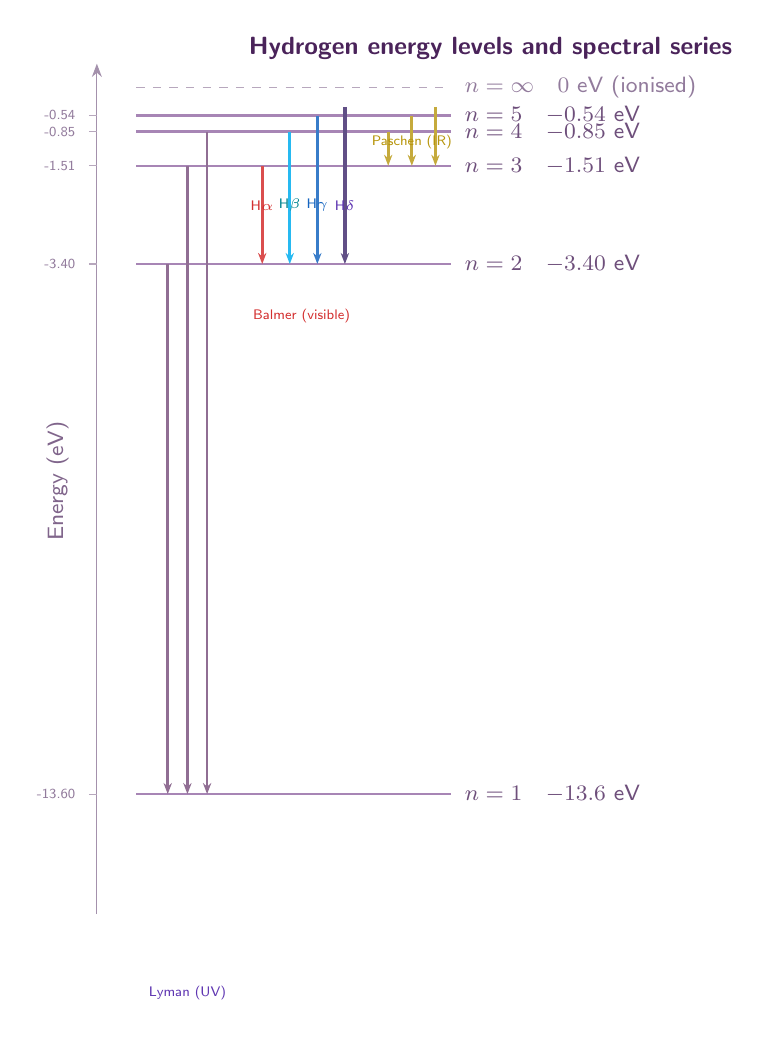
\begin{tikzpicture}[every node/.style={font=\sffamily\small}, scale=1.0]

  \node[font=\sffamily\small\bfseries, color=JourneyColor]
    at (4.5, 0.5) {Hydrogen energy levels and spectral series};

  % Energy axis
  \draw[-{Stealth}, thin, JourneyColor!50]
    (-0.5,-10.5) -- (-0.5, 0.3);
  \node[rotate=90, font=\sffamily\footnotesize, text=JourneyColor!70]
    at (-1.0,-5.0) {Energy (eV)};

  % Energy levels (scaled: E_n = -13.6/n^2)
  % n=1: -13.6 eV  -> y=-9.0 (scale: y = E*0.66)
  % n=2: -3.4  eV  -> y=-2.25
  % n=3: -1.51 eV  -> y=-1.0
  % n=4: -0.85 eV  -> y=-0.56
  % n=5: -0.54 eV  -> y=-0.36
  % inf: 0          -> y=0

  \pgfmathsetmacro{\sc}{0.66}

  \foreach \n/\E/\lbl in {
    1/-13.60/{$n=1$\quad $-13.6$ eV},
    2/-3.40/{$n=2$\quad $-3.40$ eV},
    3/-1.51/{$n=3$\quad $-1.51$ eV},
    4/-0.85/{$n=4$\quad $-0.85$ eV},
    5/-0.54/{$n=5$\quad $-0.54$ eV}
  }{
    \pgfmathsetmacro{\y}{\E*\sc}
    \draw[thick, ModuleColor!60] (0, \y) -- (4.0, \y);
    \node[right, font=\sffamily\footnotesize, text=JourneyColor!80]
      at (4.05, \y) {\lbl};
    % tick on axis
    \draw[thin, JourneyColor!40] (-0.6, \y) -- (-0.5, \y);
    \node[left, font=\sffamily\tiny, text=JourneyColor!60]
      at (-0.65, \y) {\E};
  }

  % Ionisation limit
  \draw[dashed, thin, JourneyColor!40] (0,0) -- (4.0, 0);
  \node[right, font=\sffamily\footnotesize, text=JourneyColor!60]
    at (4.05, 0) {$n=\infty$\quad $0$ eV (ionised)};

  % ── Lyman series (to n=1) ──────────────────────────────────────────────
  \pgfmathsetmacro{\yOne}{-13.60*\sc}
  \foreach \ntop/\col/\xcol in {2/blue!50!red/0.4, 3/blue!50!red/0.65,
                                  4/blue!50!red/0.9}{
    \pgfmathsetmacro{\yTop}{-13.6/(\ntop*\ntop)*\sc}
    \draw[-{Stealth[length=4pt]}, thick, \col!80, line width=1pt]
      (\xcol, \yTop) -- (\xcol, \yOne);
  }
  \node[font=\sffamily\tiny, text=blue!50!red]
    at (0.65, -11.5) {Lyman (UV)};

  % ── Balmer series (to n=2) ─────────────────────────────────────────────
  \pgfmathsetmacro{\yTwo}{-3.40*\sc}
  \pgfmathsetmacro{\yThreeB}{-13.6/(3*3)*\sc}
  \pgfmathsetmacro{\yFourB}{-13.6/(4*4)*\sc}
  \pgfmathsetmacro{\yFiveB}{-13.6/(5*5)*\sc}
  \pgfmathsetmacro{\ySixB}{-13.6/(6*6)*\sc}
  \draw[-{Stealth[length=4pt]}, thick, red!85, line width=1.2pt]
    (1.60, \yThreeB) -- (1.60, \yTwo);
  \draw[-{Stealth[length=4pt]}, thick, cyan!85, line width=1.2pt]
    (1.95, \yFourB) -- (1.95, \yTwo);
  \draw[-{Stealth[length=4pt]}, thick, blue!85, line width=1.2pt]
    (2.30, \yFiveB) -- (2.30, \yTwo);
  \draw[-{Stealth[length=4pt]}, thick, blue!60!red, line width=1.2pt]
    (2.65, \ySixB) -- (2.65, \yTwo);
  \node[font=\sffamily\tiny, text=red]
    at (2.1, -2.9) {Balmer (visible)};

  % Labels for Balmer lines
  \node[font=\sffamily\tiny, text=red] at (1.6,-1.5) {H$\alpha$};
  \node[font=\sffamily\tiny, text=cyan!80!black] at (1.95,-1.5) {H$\beta$};
  \node[font=\sffamily\tiny, text=blue] at (2.30,-1.5) {H$\gamma$};
  \node[font=\sffamily\tiny, text=blue!50!red] at (2.65,-1.5) {H$\delta$};

  % ── Paschen series (to n=3) ────────────────────────────────────────────
  \pgfmathsetmacro{\yThree}{-1.51*\sc}
  \foreach \ntop/\xcol in {4/3.2, 5/3.5, 6/3.8}{
    \pgfmathsetmacro{\yTop}{-13.6/(\ntop*\ntop)*\sc}
    \draw[-{Stealth[length=4pt]}, thick, DiscoveryColor!80, line width=1pt]
      (\xcol, \yTop) -- (\xcol, \yThree);
  }
  \node[font=\sffamily\tiny, text=DiscoveryColor]
    at (3.5,-0.7) {Paschen (IR)};

\end{tikzpicture}
\end{center}

\vspace{0.5em}

This diagram encodes everything about the hydrogen spectrum.
Each arrow represents one spectral line.
The length of the arrow is proportional to the photon energy.
The colour of the arrow corresponds approximately to the
colour of the emitted light.

\begin{problembox}
\begin{enumerate}[label=\textbf{\arabic*.}]
  \item Calculate the wavelength and energy (in eV) of the
        photon emitted in each of the following hydrogen transitions:
        \begin{enumerate}[label=(\alph*)]
          \item $n=3 \to n=2$ (H$\alpha$, Balmer)
          \item $n=4 \to n=2$ (H$\beta$, Balmer)
          \item $n=2 \to n=1$ (first Lyman line)
          \item $n=3 \to n=1$ (second Lyman line)
          \item $n=4 \to n=3$ (first Paschen line)
        \end{enumerate}
        Use $E_n = -13.6/n^2$ eV and $E_\text{photon} = hc/\lambda$
        with $hc = 1240$ eV$\cdot$nm.

  \item The \textbf{ionisation energy} of hydrogen is the energy
        needed to remove the electron from the ground state ($n=1$)
        to infinity ($n=\infty$).
        \begin{enumerate}[label=(\alph*)]
          \item Calculate the ionisation energy of hydrogen in eV.
          \item What wavelength of light is needed to ionise
                hydrogen from the ground state?
          \item Could visible light ionise hydrogen?
                What about ultraviolet light ($\lambda < 91.2$ nm)?
        \end{enumerate}

  \item A hydrogen atom absorbs a photon and jumps from $n=2$
        to $n=4$.
        \begin{enumerate}[label=(\alph*)]
          \item Calculate the energy of the absorbed photon.
          \item The atom then drops from $n=4$ to $n=2$ directly.
                What is emitted?
          \item Instead, the atom drops $n=4 \to n=3$,
                then $n=3 \to n=2$.
                Calculate the energy of each emitted photon.
          \item Add up the energies in (c). Compare to (b).
                What principle does this illustrate?
        \end{enumerate}

  \item \textbf{Helium-like systems.}
        The Rydberg formula works for any one-electron ion.
        For a nucleus with atomic number $Z$, the energy levels are:
        \[
          E_n = -\frac{13.6 Z^2}{n^2}\ \text{eV}
        \]
        \begin{enumerate}[label=(\alph*)]
          \item Calculate the ionisation energy of
                \ce{He+} ($Z=2$, one electron removed from helium).
          \item Calculate the wavelength of the $n=2 \to n=1$
                transition in \ce{He+}.
                Is this in the UV, visible, or IR?
          \item Predict the ionisation energy of \ce{Li^{2+}}
                ($Z=3$, lithium with two electrons removed).
        \end{enumerate}
\end{enumerate}
\end{problembox}

% ─── Section: Absorption Spectra ─────────────────────────────────────────────
\subsection{Absorption Spectra: The Reverse of Emission}

So far we have discussed \emph{emission} spectra:
light emitted by excited atoms.
There is a complementary phenomenon: \newterm{absorption spectra}.

When white light passes through cold hydrogen gas,
the atoms absorb photons at exactly the same wavelengths
they would emit.
The transmitted spectrum shows dark lines at those wavelengths ---
the colours missing from the continuum.

\begin{center}
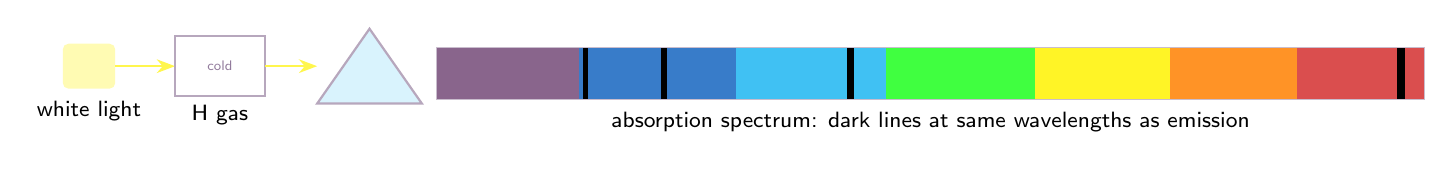
\begin{tikzpicture}[every node/.style={font=\sffamily\footnotesize}, scale=0.95]

  % White light + gas + prism schematic
  \fill[yellow!30, rounded corners=2pt] (-6.5,-0.3) rectangle (-5.8,0.3);
  \node at (-6.15,-0.6) {white light};

  \draw[-{Stealth}, thick, yellow!70] (-5.8,0) -- (-5.0,0);

  % Gas cell
  \draw[thick, JourneyColor!40] (-5.0,-0.4) rectangle (-3.8,0.4);
  \node at (-4.4,-0.65) {H gas};
  \node[font=\sffamily\tiny, text=JourneyColor!60] at (-4.4,0.0) {cold};

  \draw[-{Stealth}, thick, yellow!70] (-3.8,0) -- (-3.1,0);

  % Prism
  \fill[cyan!15] (-3.1,-0.5) -- (-2.4,0.5) -- (-1.7,-0.5) -- cycle;
  \draw[JourneyColor!40, thick] (-3.1,-0.5) -- (-2.4,0.5) -- (-1.7,-0.5) -- cycle;

  % Output: absorption spectrum
  % Rainbow bands for absorption spectrum
  \fill[blue!50!red!85]   (-1.5,-0.45) rectangle (0.4,  0.25);
  \fill[blue!85]     (0.4, -0.45) rectangle (2.5,  0.25);
  \fill[cyan!75]     (2.5, -0.45) rectangle (4.5,  0.25);
  \fill[green!75]    (4.5, -0.45) rectangle (6.5,  0.25);
  \fill[yellow!85]   (6.5, -0.45) rectangle (8.3,  0.25);
  \fill[orange!85]   (8.3, -0.45) rectangle (10.0, 0.25);
  \fill[red!85]      (10.0,-0.45) rectangle (11.7, 0.25);
  % Dark absorption lines on top
  \fill[black] (11.34,-0.45) rectangle (11.44, 0.25); % H-alpha 656nm
  \fill[black] (3.98,-0.45)  rectangle (4.08,  0.25); % H-beta 486nm
  \fill[black] (1.50,-0.45)  rectangle (1.58,  0.25); % H-gamma 434nm
  \fill[black] (0.45,-0.45)  rectangle (0.52,  0.25); % H-delta 410nm
  \draw[JourneyColor!30] (-1.5,-0.45) rectangle (11.7,0.25);
  \node at (5.1,-0.75) {absorption spectrum: dark lines at same wavelengths as emission};

\end{tikzpicture}
\end{center}

\vspace{0.5em}

The \newterm{Fraunhofer lines} in the solar spectrum are
absorption lines.
Sunlight passes through the cooler outer layers of the sun
(the chromosphere), where atoms absorb specific wavelengths.
By analysing the dark lines in sunlight,
we can determine the chemical composition of the sun ---
without ever going there.

\begin{historybox}
\textbf{Helium: Discovered on the Sun Before Earth}

In 1868, astronomers studying a solar eclipse detected
an absorption line in sunlight at 587.5 nm ---
a wavelength that did not match any known element.
They named the unknown element \emph{helium}, after Helios,
the Greek god of the sun.

It was not until 1895 that William Ramsay detected helium
in a uranium mineral on Earth.

This is the only element to have been discovered in
space before on Earth.
It was found by spectroscopy alone --- by reading the
fingerprint of its spectral lines.
\end{historybox}

% ─── Section: The Physical Meaning of n ─────────────────────────────────────
\subsection{What Does $n$ Mean Physically?}

We have established:
\begin{itemize}[nosep, leftmargin=2em]
  \item Hydrogen has discrete energy levels $E_n = -13.6/n^2$ eV.
  \item Spectral lines arise from transitions between levels.
  \item The integers $n = 1, 2, 3, \ldots$ label the levels.
\end{itemize}

But what is $n$ \emph{physically}?
The Rydberg formula forces $n$ to be an integer,
but gives no explanation for why.

In 1913, Niels Bohr proposed a model that gave $n$
a physical meaning: it counts the number of
\emph{allowed wavelengths} that fit around the electron's orbit.

This is the subject of Module~2.5.
But before accepting Bohr's model, notice something remarkable
about the data alone.

\begin{puzzlebox}
Consider the energy level diagram for hydrogen.

\begin{enumerate}[label=(\alph*), leftmargin=*]
  \item The ground state is $n=1$ with energy $-13.6$ eV.
        The first excited state is $n=2$ with energy $-3.4$ eV.
        The energy gap between them is $10.2$ eV.

        If an atom in the ground state could only gain energy
        by absorbing photons, what wavelength photon would it need
        to reach the $n=2$ state?
        Is this UV, visible, or IR?

  \item In the flame of a candle, the temperature is about
        $T \approx 1500$ K.
        The thermal energy per particle is approximately
        $k_B T = 1.38\times10^{-23} \times 1500 \approx 2\times10^{-20}$ J
        $\approx 0.13$ eV.

        Compare this thermal energy to the $n=1 \to n=2$ gap.
        Can thermal collisions in a candle flame excite
        hydrogen atoms to $n=2$?

  \item The surface of a star has temperature $T \approx 10000$ K.
        Calculate $k_B T$ in eV.
        Can thermal collisions at this temperature excite
        hydrogen atoms significantly?

  \item The Balmer series (visible lines) requires electrons
        in the $n=2$ state.
        From your answers to (b) and (c), explain why
        Balmer absorption lines are seen in stars but
        \emph{not} in cooler objects like candles.
\end{enumerate}
\end{puzzlebox}

% ─── Section: Emission from Other Elements ───────────────────────────────────
\subsection{Other Elements: More Complex, Same Principle}

Hydrogen is the simplest case --- one proton, one electron.
Its spectrum is described exactly by a single formula.

Other elements have more electrons, and their spectra are
far more complex.
But the principle is the same: each atom has discrete
energy levels, and spectral lines correspond to transitions.

\begin{center}
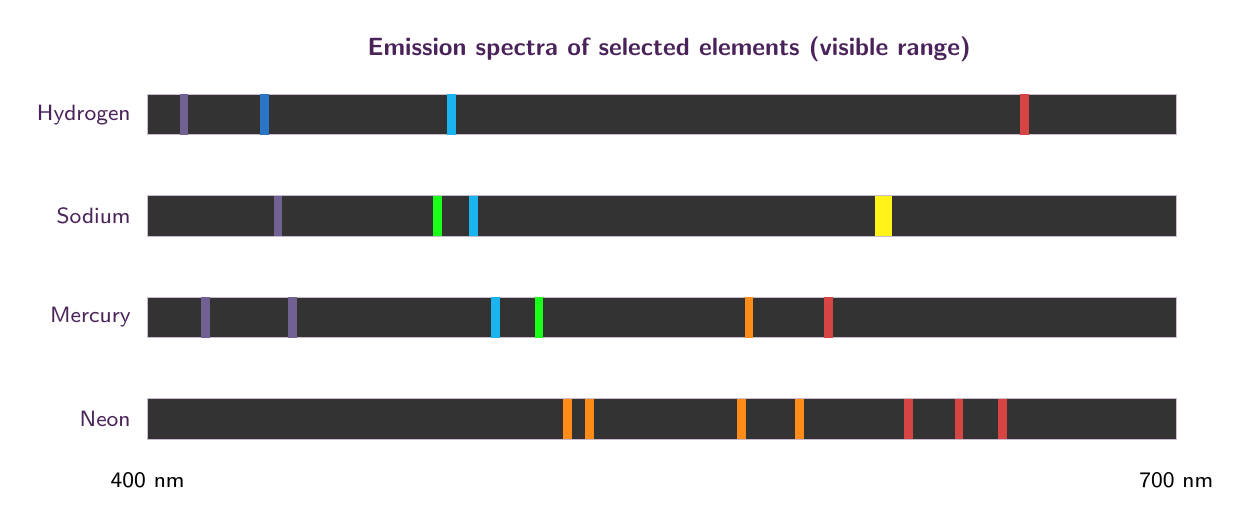
\begin{tikzpicture}[every node/.style={font=\sffamily\footnotesize}, scale=0.92]
  % Element spectra comparison
  \node[font=\sffamily\small\bfseries, color=JourneyColor] at (7.2, 5.8)
    {Emission spectra of selected elements (visible range)};

  \foreach \elem/\y/\lines in {
    Hydrogen/4.9/{
      (12.10,red),(4.19,cyan!80!black),(1.61,blue),(0.50,blue!50!red)
    },
    Sodium/3.5/{
      (10.1,yellow),(10.16,yellow),(4.5,cyan!80!black),(4.0,green),(1.8,blue!50!red)
    },
    Mercury/2.1/{
      (9.4,red),(8.3,DiscoveryColor),(5.4,green!80!black),(4.8,cyan!80!black),
      (2.0,blue!50!red),(0.8,blue!50!red)
    },
    Neon/0.7/{
      (11.8,red),(11.2,red),(10.5,red),(9.0,DiscoveryColor),
      (8.2,DiscoveryColor),(6.1,DiscoveryColor),(5.8,DiscoveryColor)
    }
  }{
    % Dark background strip
    \fill[black!80] (0,\y-0.28) rectangle (14.2,\y+0.28);
    \draw[JourneyColor!30] (0,\y-0.28) rectangle (14.2,\y+0.28);
    \node[anchor=east, text=JourneyColor] at (-0.1,\y) {\elem};
  }

  % Draw lines for each element (Hydrogen)
  \fill[red!90]          (12.04,4.62) rectangle (12.16,5.18);
  \fill[cyan!90]         (4.13, 4.62) rectangle (4.25, 5.18);
  \fill[blue!90]         (1.55, 4.62) rectangle (1.67, 5.18);
  \fill[blue!60!red!90]  (0.44, 4.62) rectangle (0.56, 5.18);
  % Sodium
  \fill[yellow!90]       (10.04,3.22) rectangle (10.16,3.78);
  \fill[yellow!90]       (10.16,3.22) rectangle (10.28,3.78);
  \fill[cyan!90]         (4.44, 3.22) rectangle (4.56, 3.78);
  \fill[green!90]        (3.94, 3.22) rectangle (4.06, 3.78);
  \fill[blue!60!red!90]  (1.74, 3.22) rectangle (1.86, 3.78);
  % Mercury
  \fill[red!90]          (9.34, 1.82) rectangle (9.46, 2.38);
  \fill[orange!90]       (8.24, 1.82) rectangle (8.36, 2.38);
  \fill[green!90]        (5.34, 1.82) rectangle (5.46, 2.38);
  \fill[cyan!90]         (4.74, 1.82) rectangle (4.86, 2.38);
  \fill[blue!60!red!90]  (1.94, 1.82) rectangle (2.06, 2.38);
  \fill[blue!60!red!90]  (0.74, 1.82) rectangle (0.86, 2.38);
  % Neon
  \fill[red!90]     (11.74,0.42) rectangle (11.86,0.98);
  \fill[red!90]     (11.14,0.42) rectangle (11.26,0.98);
  \fill[red!90]     (10.44,0.42) rectangle (10.56,0.98);
  \fill[orange!90]  (8.94, 0.42) rectangle (9.06, 0.98);
  \fill[orange!90]  (8.14, 0.42) rectangle (8.26, 0.98);
  \fill[orange!90]  (6.04, 0.42) rectangle (6.16, 0.98);
  \fill[orange!90]  (5.74, 0.42) rectangle (5.86, 0.98);

  % Wavelength axis
  \node at (0,-0.15) {400 nm};
  \node at (14.2,-0.15) {700 nm};

\end{tikzpicture}
\end{center}

\vspace{0.5em}

Notice that each element has a unique pattern.
Sodium's two bright yellow lines (the sodium doublet at 589 nm)
are responsible for the orange glow of sodium street lamps.
Neon's many red-orange lines give neon signs their characteristic
colour.
Mercury's strong lines in the blue-green and ultraviolet
make mercury-vapour lamps appear blueish-white.

Every line corresponds to a specific transition between
energy levels specific to that element.
\emph{Spectroscopy is the direct observation of atomic
energy levels.}

% ─── Section: Where This Leads ───────────────────────────────────────────────
\subsection{What the Spectrum Demands of Any Theory}

Any correct theory of the atom must explain:

\begin{enumerate}[leftmargin=2em]
  \item Why energy levels exist at all --- why atoms cannot have
        arbitrary energies.
  \item Why the levels for hydrogen follow the $1/n^2$ law.
  \item Why the quantum number $n$ must be a positive integer.
  \item Why the ground state ($n=1$) is stable ---
        why the electron does not fall further.
  \item How to calculate the Rydberg constant $R_H$ from
        more fundamental quantities.
\end{enumerate}

Bohr's model (Module~2.5) will explain all five.
Wave mechanics (Module~2.6) will explain \emph{why}
Bohr's model works.

% ─── Section: Deep Problems ──────────────────────────────────────────────────
\subsection*{Deep Problems}

\begin{deepbox}
\begin{enumerate}[label=\textbf{D\arabic*.}]

  \item \textbf{The Rydberg Constant from First Principles.}

        Bohr's model (derived in Module~2.5) gives:
        \[
          R_H = \frac{m_e e^4}{8 \varepsilon_0^2 h^3 c}
        \]
        \begin{enumerate}[label=(\alph*)]
          \item Check that this expression has the correct
                dimensions of m$^{-1}$.
          \item Substitute numerical values:
                $m_e = 9.109\times10^{-31}$ kg,
                $e = 1.602\times10^{-19}$ C,
                $\varepsilon_0 = 8.854\times10^{-12}$ C$^2$N$^{-1}$m$^{-2}$,
                $h = 6.626\times10^{-34}$ Js,
                $c = 2.998\times10^8$ ms$^{-1}$.
          \item Compare your result to the measured value
                $R_H = 1.0974\times10^7$ m$^{-1}$.
          \item The fact that this formula, derived from
                theoretical principles, reproduces the
                measured Rydberg constant to five significant
                figures was one of the strongest validations
                of the Bohr model.
                Why is this kind of quantitative agreement
                more compelling than a qualitative description?
        \end{enumerate}

  \item \textbf{Stellar Classification by Spectra.}

        Stars are classified by their spectra into types
        O, B, A, F, G, K, M (hottest to coolest).
        The strength of absorption lines depends on
        the fraction of atoms in the required initial state.

        For Balmer absorption lines (which require $n=2$),
        the fraction of hydrogen in $n=2$ is proportional to:
        \[
          f_2 \propto e^{-E_2/k_BT} = e^{+3.4/k_BT\ \text{(eV)}}
        \]
        (More precisely, the Boltzmann factor $e^{-\Delta E/k_BT}$
        gives the probability of a state with energy $\Delta E$
        above the ground state.)

        \begin{enumerate}[label=(\alph*)]
          \item The energy gap from $n=1$ to $n=2$ is 10.2 eV.
                Calculate the Boltzmann factor $e^{-10.2/k_BT}$
                at $T = 5800$ K (Sun), $T = 10000$ K (A-type star),
                $T = 25000$ K (B-type star).
                Use $k_B = 8.617\times10^{-5}$ eV/K.
          \item Which star type should show the strongest
                Balmer lines?
          \item At very high temperatures ($T > 30000$ K),
                hydrogen becomes fully ionised.
                What happens to the Balmer lines?
          \item At very low temperatures ($T < 4000$ K),
                almost no hydrogen is in $n=2$.
                What happens to the Balmer lines?
          \item Explain why Balmer lines are strongest at
                intermediate temperatures, and sketch a curve
                of Balmer line strength vs temperature.
        \end{enumerate}

  \item \textbf{Franck-Hertz Experiment: Confirming Energy Levels.}

        In 1914, James Franck and Gustav Hertz bombarded mercury
        vapour with electrons of controllable energy.
        They measured the current reaching a collector as a
        function of the electron energy (accelerating voltage).

        They found: the current rose smoothly, then dropped
        sharply at $V = 4.9$ V, rose again, dropped at $9.8$ V,
        rose, dropped at $14.7$ V, and so on.

        \begin{enumerate}[label=(\alph*)]
          \item Interpret the current drops.
                What is happening to the electrons at $4.9$ V?
          \item Why does the pattern repeat at multiples of 4.9 V?
          \item Mercury has a strong emission line at 253.7 nm.
                Calculate the energy of this photon in eV.
                Compare to 4.9 eV.
          \item Why is the Franck-Hertz experiment
                considered direct proof of discrete energy levels,
                independent of spectroscopy?
          \item What would you observe if energy levels were
                \emph{continuous} rather than discrete?
        \end{enumerate}

\end{enumerate}
\end{deepbox}

% ─── Reflection ──────────────────────────────────────────────────────────────
\subsection*{Reflection}

\begin{reflectionbox}
\begin{enumerate}[label=\textbf{R\arabic*.}]
  \item Balmer found his formula by staring at four numbers
        for a few weeks.
        Rydberg generalised it to all hydrogen series.
        Both were purely empirical --- pattern recognition
        without physical understanding.
        \textbf{What is the role of empirical pattern-finding
        in physics?} Is it ``real'' science, or just
        the precursor to real science?

  \item The Fraunhofer lines in sunlight revealed the
        composition of the sun from Earth.
        Spectroscopy of distant galaxies allows us to measure
        their composition, temperature, and velocity.
        \textbf{What does it mean that the laws of physics ---
        including quantum energy levels --- appear to be the
        same throughout the observable universe?}
        Could they be different somewhere, and how would we know?

  \item The Rydberg formula uses two integers $n_1$ and $n_2$.
        \textbf{Why are the quantum numbers integers rather
        than fractions or irrational numbers?}
        What physical constraint forces discreteness?
        Write your best hypothesis (Module~2.5 will answer it).

  \item When hydrogen emits a photon and drops from $n=4$ to $n=2$,
        it emits exactly one photon with exactly the right energy.
        \textbf{How does the atom ``know'' which transition to make,
        and when?} Is there a mechanism, or is it fundamentally random?
        What does your answer imply about determinism in nature?
\end{enumerate}
\end{reflectionbox}

\vspace{1.5em}
\begin{center}
\begin{tcolorbox}[enhanced, colback=DiscoveryColor!8, colframe=DiscoveryColor,
  width=0.88\textwidth, arc=3pt]
\centering\sffamily\small
\textbf{What we invented in this module.}\\[4pt]
We invented the concept of discrete atomic energy levels.
Not by assuming them, but by being forced into them by data.
The hydrogen spectrum --- four lines, measured to six significant
figures, fitting a formula with two integers --- leaves no room
for continuous energy.
The integers demand quantisation.
The $1/n^2$ law demands a specific formula for the levels.
And the convergence of series toward finite limits demands
a ground state from which no further emission is possible.
All of this is in the data.
All of it was there waiting since 1885.
We needed Bohr to hear what the data was saying.
\end{tcolorbox}
\end{center}

\vspace{2em}
\noindent\textcolor{JourneyColor!40}{\rule{\textwidth}{0.6pt}}
\begin{center}
\textit{\sffamily\small
Module 2.4 complete. Continue to Module 2.5:\\
\textbf{Bohr's Model: Quantised Orbits}.}
\end{center}

\end{document}